\documentclass[fontsize=17pt]{extarticle}
% !TeX spellcheck = en_GB 
\renewcommand{\baselinestretch}{1.5}
\usepackage{array,tabularx}
\usepackage{arxiv}
\usepackage{amsmath}
\newenvironment{conditions*}
{\par\vspace{\abovedisplayskip}\noindent
	\tabularx{\columnwidth}{>{$}l<{$} @{${}\longmapsto{}$} >{\raggedright\arraybackslash}X}}
{\endtabularx\par\vspace{\belowdisplayskip}}
\usepackage{fontawesome}
\usepackage[utf8]{inputenc} % allow utf-8 input
\usepackage[T1]{fontenc}    % use 8-bit T1 fonts
\usepackage{hyperref}       % hyperlinks
\usepackage{url}            % simple URL typ
\usepackage{booktabs}       % professional-quality tables
\usepackage{amsfonts}       % blackboard math symbols
\usepackage{nicefrac}       % compact symbols for 1/2, etc.
\usepackage{microtype}      % microtypography
\usepackage{lipsum}
\usepackage[utf8]{inputenc} % Required for inputting international characters
\usepackage[T1]{fontenc} % Output font encoding for international characters
\usepackage{pgfplots}
\usepackage{graphicx}
\usepackage{fancyhdr}
\usepackage{mathpazo} % Palatino font
\hypersetup{%
	pdfborder = {0 0 0}
}

%Handling Keywords
\def\keywordname{{\bfseries \emph Keywords}}%
\def\keywords#1{\par\addvspace\medskipamount{\rightskip=0pt plus1cm
		\def\and{\ifhmode\unskip\nobreak\fi\ $\cdot$
		}\noindent\keywordname\enspace\ignorespaces#1\par}}
	
\usepackage[T1]{fontenc}
\usepackage[utf8]{inputenc}
\usepackage{charter}
\usepackage{environ}
\usepackage{tikz}
\usetikzlibrary{calc,matrix}

%%%%%%%%%%%%%%%%%%%%%%%%%%%%%%%%%%
%For Timeline
%%%%%%%%%%%%%%%%%%%%%%%%%%%%%%%%%%
\makeatletter
\let\matamp=&
\catcode`\&=13
\makeatletter
\def&{\iftikz@is@matrix
	\pgfmatrixnextcell
	\else
	\matamp
	\fi}
\makeatother

\newcounter{lines}
\def\endlr{\stepcounter{lines}\\}

\newcounter{vtml}
\setcounter{vtml}{0}

\newif\ifvtimelinetitle
\newif\ifvtimebottomline
\tikzset{description/.style={
		column 2/.append style={#1}
	},
	timeline color/.store in=\vtmlcolor,
	timeline color=red!80!black,
	timeline color st/.style={fill=\vtmlcolor,draw=\vtmlcolor},
	use timeline header/.is if=vtimelinetitle,
	use timeline header=false,
	add bottom line/.is if=vtimebottomline,
	add bottom line=false,
	timeline title/.store in=\vtimelinetitle,
	timeline title={},
	line offset/.store in=\lineoffset,
	line offset=4pt,
}

\NewEnviron{vtimeline}[1][]{%
	\setcounter{lines}{1}%
	\stepcounter{vtml}%
	\begin{tikzpicture}[column 1/.style={anchor=east},
	column 2/.style={anchor=west},
	text depth=0pt,text height=1ex,
	row sep=1ex,
	column sep=1em,
	#1
	]
	\matrix(vtimeline\thevtml)[matrix of nodes]{\BODY};
	\pgfmathtruncatemacro\endmtx{\thelines-1}
	\path[timeline color st] 
	($(vtimeline\thevtml-1-1.north east)!0.5!(vtimeline\thevtml-1-2.north west)$)--
	($(vtimeline\thevtml-\endmtx-1.south east)!0.5!(vtimeline\thevtml-\endmtx-2.south west)$);
	\foreach \x in {1,...,\endmtx}{
		\node[circle,timeline color st, inner sep=0.15pt, draw=white, thick] 
		(vtimeline\thevtml-c-\x) at 
		($(vtimeline\thevtml-\x-1.east)!0.5!(vtimeline\thevtml-\x-2.west)$){};
		\draw[timeline color st](vtimeline\thevtml-c-\x.west)--++(-3pt,0);
	}
	\ifvtimelinetitle%
	\draw[timeline color st]([yshift=\lineoffset]vtimeline\thevtml.north west)--
	([yshift=\lineoffset]vtimeline\thevtml.north east);
	\node[anchor=west,yshift=16pt,font=\large]
	at (vtimeline\thevtml-1-1.north west) 
	{
	%\textsc{Timeline \thevtml}:
	\textit{\vtimelinetitle}};
	\else%
	\relax%
	\fi%
	\ifvtimebottomline%
	\draw[timeline color st]([yshift=-\lineoffset]vtimeline\thevtml.south west)--
	([yshift=-\lineoffset]vtimeline\thevtml.south east);
	\else%
	\relax%
	\fi%
	\end{tikzpicture}
}
%%%%%%%%%%%%%%%%%%%%%%%%%%%%%%%%%%%%%%%%%%%%

\fancyhf{}
%\fancyhead[LE,RO]{Prudent Valuation: IR Delta Concentration}
\fancyhead[RE,LO]{\raisebox{1.3\height}\leftmark}
%\fancyhead[RE,RO]{
\includegraphics[scale=0.02]{db.png}}
%\fancyfoot[CE,LO]{\leftmark}
\fancyfoot[LE,CO]{Page \thepage}
\graphicspath{{_images_tables_figures/}}
\title{Change of Probability Measure\\
	\emph{Part1: Normal Variables} }

\author{
	Ali~Al-Hayki\thanks{Use footnote for providing further
		information about author (webpage, alternative
		address)---\emph{not} for acknowledging funding agencies.} \\
	\faEnvelopeO \quad \href{mailto:ali.hayki@gmail.com}{\nolinkurl{
			ali.hayki@gmail.com} }\\
	\faGithub \quad \texttt{\href{https://github.com/hayki}{alihayki}}\\
	\faLinkedin \quad \texttt{\href{https://linedin.com/in/ali-al-hayki-17baa180/}{ali-al-hayki}}\\
}
\date{01/02/2020}

\begin{document}
	
\maketitle



\begin{figure}
	\begin{center}
	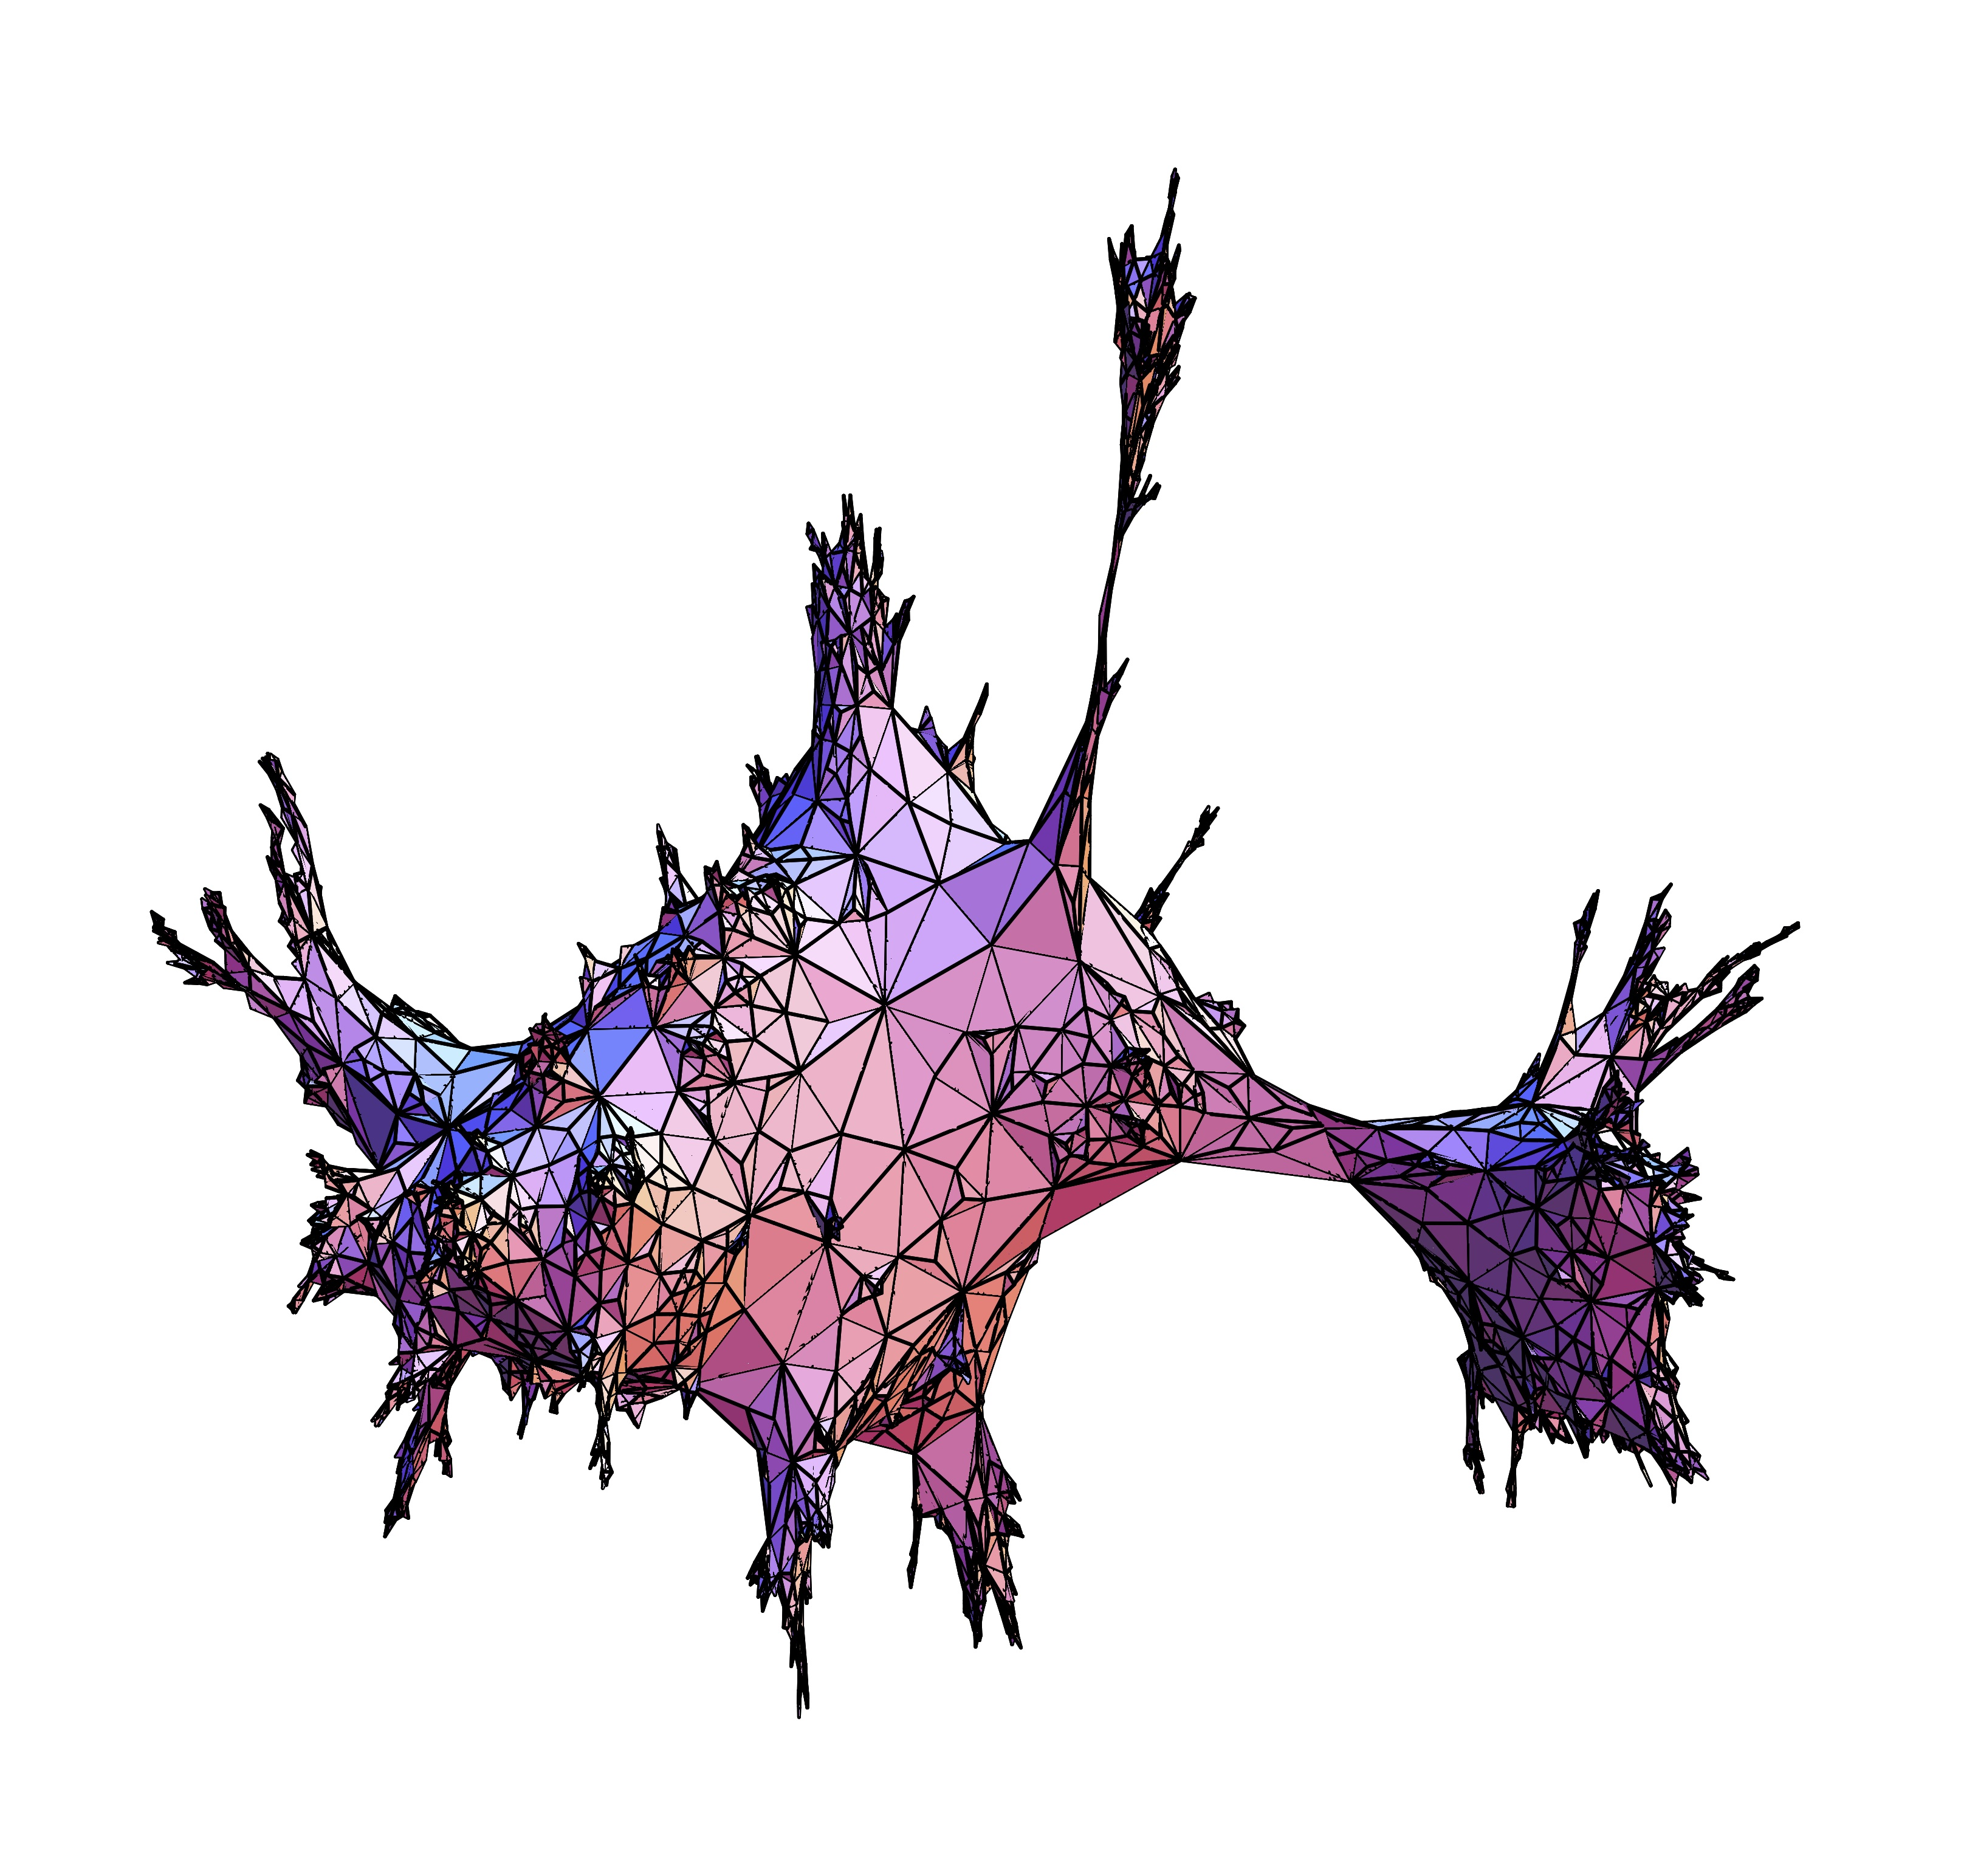
\includegraphics[scale=0.4]{sur5.jpg}\\[0.5cm]
\end{center}
\end{figure}

\newpage
\begin{abstract}
The purpose of this paper is to help students and professionals, who have introductory knowledge of quantitative finance, to develop more advanced knowledge and skills that one needs in order to follow advanced literature, and to build/appreciate models used in trading, pricing, and risk management. The transition from introductory to advanced is the most rewarding, but is one of the hardest steps in the development of a quant and I am aiming to help you with this transition.

This paper will particularly develop the concept of change of probability measure using normal distribution as an example. It Introduces the technical concepts under the simplest possible settings, which will then be applied to finite stochastic process and Brownian motion. 
\end{abstract}


% keywords can be removed
\keywords{First keyword \and Second keyword \and More}


\tableofcontents
\newpage



\section{Introduction}

In this paper we are going to explain the change of of probability measure which is one of the simplest yet one of the most powerful concepts with far-reaching consequences. It is also one of the most commonly tested concepts in job interviews. We are going to develop the concept using standard normal distribution. Later we will change the settings to a finite dimensional stochastic process which will be easy because by then we would have learned the tricks of the trade. This will lead us nicely to the Cameron-Martin-Girsanov Theorem for Brownian Motion. We will then give some examples of its uses such as changing the drift of a process, evaluating truncated conditional expectation using derivations of Black-Scholes formula as an example and importance sampling.

\section{Normal Distribution}
Lets start with a simple Normally distributed random variable. Assume that a variable under a given probability measure, \textit{P}, follows a standard normal distribution:

\begin{center}
$X$ under $P\sim N[0,1]$
\end{center}

Recall the formula of the \textit{density function} a standard normal is:

\begin{equation}
p(x)=\frac{1}{\sqrt{2\pi}}e^{-\frac{1}{2}x^{2}}
\end{equation}

the distribution function which gives the probability of the random variable taking values less than a certain value, say X, can be written as the integral of the density function:

\begin{equation}
P(x)=P[X\leq x]=\int_{-\infty}^{x}p(t)dt
\end{equation}

we can write the write the relationship in differential form as well:

\begin{equation}
dP(x)=p(x)dx
\end{equation}

Now the distribution function is essentially a probability measure because it gives probability of events which in the present case are intervals for example we can write the probability that the value of the random variable is between alpha and beta as follows:

\begin{equation}\label{equ: SND}
P[\alpha \leq X \leq \beta]=\frac{1}{\sqrt{2\pi}}\int_{\alpha}^{\beta}e^{-\frac{1}{2}x^{2}}dx
\end{equation}
\pgfmathdeclarefunction{gauss}{2}{%
	\pgfmathparse{1/(#2*sqrt(2*pi))*exp(-((x-#1)^2)/(2*#2^2))}%
}

So the change of the distribution function on the same random variable is nothing but an example of a probability measure change, to see this let's assume that we shift the interval by a constant:
\begin{equation}\label{equ: ShiftedSND}
P[\alpha-\mu \leq X \leq \beta-\mu]=\frac{1}{\sqrt{2\pi}}\int_{\alpha-\mu}^{\beta-\mu}e^{-\frac{1}{2}x^{2}}dx
\end{equation}

Essentially we shifted the lower and the upper integration limits by the same constants leaving the random variable X untouched - \textbf{Leaving the variable unchanged is the main trick!}. Now lets preform a change of variable so the interval of integration gets aligned to equation \ref{equ: SND}. \textit{Think of this as an attempt to determine how much shift in the probability of the original interval has been induced by the given shift of the integration interval}. Lets define a new variable $y=x+\mu$. when x equals the lower integration limit $=\alpha-\mu$ then Y becomes $\alpha$:
\begin{equation}
y=\alpha-\mu +\mu=\alpha
\end{equation}
Analogously when x equals the upper integration limit $=\beta-\mu$then Y becomes $\beta$:
\begin{equation}
y=\beta-\mu +\mu=\beta
\end{equation}
Finally, $x=\mu$ and taking the derivative with respect to y we get $dx=dy$. Making the substitutions into equation \ref{equ: ShiftedSND}.
\begin{equation}\label{equ: SubSND}
P[\alpha \leq X \leq \beta]=\frac{1}{\sqrt{2\pi}}\int_{\alpha}^{\beta}e^{-\frac{1}{2}(y-\mu)^{2}}dy
\end{equation}

\textit{So the \textbf{intervals are the same} now but the \textbf{probability has shifted}}. We can call the event $P[\alpha \leq X \leq \beta]$ as event \underline{$A$}. Then the shifted event $P[\alpha-\mu \leq X \leq \beta-\mu]$ can be written as the probability of \underline{$A-\mu$}.  

We recognise this as the probability of a normal variable with mean $\mu$.

Now lets analyse this simple relationship in more detail:
\begin{equation}\label{equ: SubSND}
P[A-\mu]=P[\alpha \leq X \leq \beta]=\frac{1}{\sqrt{2\pi}}\int_{\alpha}^{\beta}e^{-\frac{1}{2}(y-\mu)^{2}}dy
\end{equation}


As y is just a dummy variable, we can switch back to x to make the comparison clearer
\begin{equation}
	 =\frac{1}{\sqrt{2\pi}}\int_{\alpha}^{\beta}e^{-\frac{1}{2}(x-\mu)^{2}}dy
\end{equation}

Expand the squares:     
\begin{equation}
=\frac{1}{\sqrt{2\pi}}\int_{\alpha}^{\beta}e^{-\frac{1}{2}(x^{2}-2x\mu+\mu^{2})}dx
\end{equation}

Spiting the exponential into 2 terms
\begin{equation}
=\frac{1}{\sqrt{2\pi}}\int_{\alpha}^{\beta}e^{-\frac{1}{2}x^{2}}e^{x\mu+-\frac{1}{2}\mu^{2}}dx
\end{equation}
The aim is isolate the standard normal density which is obvious now and we can write it in terms of the standard normal density which we denoted with small P:

\begin{equation}
=\int_{\alpha}^{\beta}e^{x\mu+-\frac{1}{2}\mu^{2}}p(x)dx
\end{equation}
 Recalling the relationship between the distribution function in differential form:

\begin{equation}\label{equ: SNDdif}
=\int_{\alpha}^{\beta}e^{x\mu+-\frac{1}{2}\mu^{2}}dP(x)
\end{equation}

We can now represent equation \ref{equ: SNDdif} in a few alternative forms which will help us with the terminology. 

\textbf{Form 1:} The interval can be denoted  in terms of its name $A$ (i.e. $\int_{\alpha}^{\beta}=\int_{A}^{}$)

\begin{equation}\label{equ: SNDevent}
=\int_{A}^{}e^{x\mu+-\frac{1}{2}\mu^{2}}dP(x)
\end{equation}

\textbf{Form 2: } The interval can also be 'indicated' using an indicator function which take a value of 1 for values of the variable within the indicated interval and 0 otherwise $1_A:X\rightarrow{\{0,1\}}$ (i.e. the indicator only activates if a certain condition is true). \footnote{If an indicator function is over a subset of random variables, then the expectation of the indicator function is the probability of that subset occurring.}

As the indicator function nullifies the domain that is outside the interval of interest, we can write the limit of integration to go from minus infinity to plus infinity

\begin{equation}
=\int_{-\infty}^{\infty}e^{x\mu+-\frac{1}{2}\mu^{2}}1_{[\alpha,\beta]}dP(x)
\end{equation} 

now this is nothing but the expected value of the exponential function times the indicator function of the event. 

\begin{equation}\label{equ: SNDInd}
=E^{P}[e^{x\mu+-\frac{1}{2}\mu^{2}}1_{A}]
\end{equation} 

The exponential is a random variable, as it is a function of x, we will denote it with the symbol $Z$,
\begin{equation}
=E^{P}[Z(x)1_{A}]
\end{equation} 

It was all very simple and trivial but will help us when we get into more complicated settings. Try to remember the steps no matter how trivial they look in the current settings.

We previously said that this shift of the interval can be viewed as leading to a change of probability so lets use it to define a new probability measure,

we can use any of the alternative forms discussed. The 2 forms that will be mostly relevant are equations \ref{equ: SNDevent} and \ref{equ: SNDInd}.

\begin{equation}\label{equ: SNDevent}
Q[A]=\int_{A}^{}e^{x\mu+-\frac{1}{2}\mu^{2}}dP(x)
\end{equation}


\subsection{Q Measure}
\begin{equation}\label{equ: SNDevent}
Q[A]=\int_{A}^{}e^{x\mu+-\frac{1}{2}\mu^{2}}dP(x)=E^{P}[Z(x)1_{A}]
\end{equation}
Lets calculate the cumulative probability of a variable taking a value below $a$,

\begin{equation}
Q[X\leq a]=E^{P}[e^{x\mu+-\frac{1}{2}\mu^{2}}1_{X\leq a}]
\end{equation}
 
 and writing the expectation in terms of the integration with respect to the probability,

 \begin{equation}
 Q[X\leq a]=\frac{1}{\sqrt{2 \pi}} \int_{-\infty}^{\infty}e^{x\mu-\frac{1}{2}\mu^{2}}1_{X\leq a}e^{-\frac{1}{2}x^{2}}dx
 \end{equation}
 
 reflecting the indicator function in the integration limit,
 
  \begin{equation}
 Q[X\leq a]=\frac{1}{\sqrt{2 \pi}} \int_{-\infty}^{a}e^{x\mu-\frac{1}{2}\mu^{2}}e^{-\frac{1}{2}x^{2}}dx
 \end{equation}
 
 Combine the 2 exponentials,
 
 
   \begin{equation}
 Q[X\leq a]=\frac{1}{\sqrt{2 \pi}} \int_{-\infty}^{a}e^{-\frac{1}{2}(-2x\mu+\mu^{2}+x^{2})}dx
 \end{equation}
 Which we recognise as a complete square,
 
    \begin{equation}
 Q[X\leq a]=\frac{1}{\sqrt{2 \pi}} \int_{-\infty}^{a}e^{-\frac{1}{2}(x-\mu)^{2}}dx
 \end{equation}
 Now this is just the distribution function of a normal variable with mean $\mu$ so it is a valid distribution function. A distribution function is a probability measure as can be easily verified by recalling the definition of the probability measure.
 
 \subsection{Probability Measure Verification}

Probability Measure: $\lambda$ 
  \begin{itemize}
 \item $0\leq\lambda(E_i)\leq1$: The probability measure of an event has to be between 0 and 1 which the distribution function satisfies.
 \item $\lambda(\phi)=0, \lambda(\Omega)=1$: The probability of the null set and the whole sample must be 0 and 1 respectively which the distribution function satisfies.
 \item $\{E_{i}\}=\{E_{1},E_{2},...\}$: If we have a list of disjoint events then the probability of their union is the sum of their probabilities 
 \begin{equation}
 \lambda\left(\bigcup E_{i}\right)=\sum\lambda(E_{i})
 \end{equation}
 \end{itemize} 
 Our $Q$ definitely satisfies this, so the $Q$ is definitely a probability measure.
 
 So we started with a probability distribution $P$:
 \begin{equation}
 X \text{ under } P \sim N[0, 1]
 \end{equation}
and we showed that shifting the interval induces a new distribution $Q$:
 \begin{equation}
X \text{ under } Q \sim N[\mu, 1]
\end{equation}

\subsection{Relationship Between P and Q Distributions}
Let's analyse the relationship between the 2 distributions now.
\begin{equation}
Q[A]=\int_{A}e^{x\mu-\frac{1}{2}\mu^{2}}dP(x)
\end{equation}

We can write the $Q$ probability of the $X$ taking values between $\alpha$ and $y$ as follows:

\begin{equation}
Q[\alpha\leq X \leq y]=\int^{y}_{\alpha}e^{x\mu-\frac{1}{2}\mu^{2}}dP(x)
\end{equation}
We can writer the left-hand side as the difference between the values of the distribution function.

\begin{equation}
Q(y)-Q(\alpha)=\int^{y}_{\alpha}z(x)dP(x)
\end{equation}


Where we use the symbol $Z$ to represent the exponential function. Now this is very similar to the fundamental therm of calculus which establishes a connection between the two central operations of calculus - integration and differentiation. We produce it in a convenient form here:

\begin{equation}
F(y)-F(a)=\int^{y}_{\alpha}f(x)dx
\end{equation} 

The small f function $f$ is the derivative of the capital f function $F$
\begin{equation}
\frac{dF(y)}{dy}=f(y)
\end{equation}
Hence the capital f function $F$ is the anti derivative or the primitive or the integral of the small $f$. You can easily see the relationship between the probability measures $Q$ and $P$ through the $Z$ function. The question we face now are what conditions are needed on the function and its derivative, that's the capital $F$ function and it derivative the small $f$ so that both sides of the above equation are defined and equal. If the derivative is continuous then the relationship between the derivative and the function is given by the fundamental theorem of calculus holds, but we would like the conditions in terms of the function itself. Requiring that the function be just continuous in the sense of the usual definition is not sufficient. It indeed sounds strange that we cannot recover the function by integrating its derivative and the derivative by differentiating its integral even if the function is continuous so the trouble must be in the continuity definition and we tighten the continuity definition then things might work out . 


\subsection{Continuity}
Recall that only a small subset of the continuous functions are differentiable between the two there are many shades of continuity:
\begin{center}
	\begin{vtimeline}[description={text width=7cm}, 
	row sep=7ex, 
	use timeline header,
	timeline title={Continuity Spectrum}]
	\color{white}- & \textbf{Continuous}\endlr 
	\color{white}- & Uniformly Continuous\endlr
	\color{white}- & Absolutely Continuous\endlr
	\color{white}- & Lipschitz Continuous\endlr
	\color{white}- & \textbf{Continuously Differentiable}\endlr
\end{vtimeline}
\end{center}

All these definitions call a function continuous if a small change in the input leads to a small change in the output but they assess them smallness differently. The requirement get tighter as one moves from the top to bottom and as such the number of functions which satisfies the criteria reduces as one moves from the top to the bottom. If the derivative is continuous then we are at the bottom end of the continuum and the relationship between the derivative and the function that is given by the fundamental therm holds. If the function is just continuous then we are at the top end of the continuum and this requirement is not sufficient for the relationship to hold. So the right answer must be in the middle. If the function is absolutely continuous then the fundamental theorem holds. Absolute continuity imposes stricter requirements from the basic continuity to get a feel for the differences in the requirements we quickly outline the definition of absolute continuity and relate it to the usual epsilon-delta definition. We will not need this technical definition as things simplify when one moves from the real line to the general measure spaces but it is good to know for context. The definition goes in the usual epsilon-delta style. A function $F(y)$ is absolutely continuous on $[a,b]$, if for every $\epsilon>0$, there is a $\delta$ such that for every finite collection of disjoint intervals $\left\{(a_{i},b_{i}), (a_{i},b_{i}), ... , (a_{i},b_{i})\right\}$ if the absolute variation of the inputs is less than Delta then the absolute variation of the function outputs is less than epsilon:

\begin{equation}
\sum_{i=1}^{n}\left|b_{i}-a_{i} \right|<\delta, \quad \quad then \quad\sum_{i=1}^{n}\left|F(b_{i})-F(a_{i}) \right|<\epsilon
\end{equation}

Setting n equal to 1 gives a definition of uniform continuity and if one is allowed to choose Delta separately based on X then one gets the usual epsilon delta definition of local continuity. The definition simplifies when one switches to measures. 
\subsection{Measure Theory}
A measure Q is said to be absolutely continuous with respect to another measure P $(Q\ll P)$ if whenever measure P assigns 0 probability to an event then Q also assigns zero probability to the same event (i.e. if $P(E)=0$ then $Q(E)=0$). In simple terms the null set under $P$ is also the null set under $Q$. Notice the absolute continuity is represented by the double less than symbol $\ll$. An easy way to remember this is to say that $Q$ is dominated by $P$ in that the null set under $P$ must be a null set under $Q$. As we know the probability measure is indeed a measure so this definition applies to probability measures as well. For the probability measure defined by the continuous distribution functions on the real line that we have been discussing so far. The 2 definitions that is the complicated looking definition above and a simple definition are equivalent, but this simple looking definition is the one that applies in more general settings. Just for completeness the reason this definition does not contain the usual epsilon-delta is because a general measure is not necessary finite and if the measure happens to be finite which should be the case for the probability measure then one recast the definition in terms of the familiar epsilon delta (i.e. if $P(E) <\delta$, then $Q(E)<\epsilon$). Though this definition is not commonly used, it is easy to check that the probability measure Q is absolutely continuous with respect to the measure P and given the similarity of the connection between the two probability measure to the fundamental theorem. It wont come as a big surprise if we call the function Z the derivative of the probability measure Q with respect to the probability measure P:
\begin{equation}
	\frac{dQ(y)}{dP(y)}=z(y)
\end{equation}
The derivative is called the Radon–Nikodym derivative in the technical literature and we shall be calling $z(y)$ the Radon–Nikodym derivative from now onwards. the so called Radon–Nikodym theorem goes a step further. If a measure Q is absolutely continuous with another measure P then it guarantees the existence and uniqueness of the function z or the derivative of the measure with respect to the other. If $Q\ll P$, then there is $z$ such that:
\begin{equation}
	Q[A]=\int z(x)dP(x) \qquad \frac{dQ(x)}{dP(x)}=z(x) 
\end{equation}
It is also called density for the obvious reasons. If P is absolutely continuous with respect to Q then we say that the two measures are equivalent and one can then switch between the two effortlessly as the Radon Radon–Nikodym applies to measures and our measure being a probability measure has to satisfy some extra conditions such as the total probability must be 1. We need to verify that the function $z$ us indeed a probability density function so we will have to check that it is non-negative and that its expected value is 1 which is the same thing as checking that the total probability sums is up to 1.
\begin{equation}\label{equ: RadNc}
z(x)=e^{x-\mu-\frac{1}{2}\mu^{2}}\ge 0
\end{equation}
as function \ref{equ: RadNc} is exponential it is non-negative by default. Now for the second requirement, let's calculate its expected value under the measure p:

\begin{equation}\label{equ: RadNc}
E^{P}\left[e^{x-\mu-\frac{1}{2}\mu^{2}}\right]=\frac{1}{\sqrt{2\pi}}\int_{-\infty}^{\infty}e^{x-\mu-\frac{1}{2}\mu^{2}}dx=\frac{1}{\sqrt{2\pi}}\int_{-\infty}^{\infty}e^{-\frac{1}{2}(x-\mu)^{2}}dx=1
\end{equation}

Thus the total probability under $Q$ will be 1 as we can verify by substituting the Radon Radon–Nikodym derivative:

\begin{equation}\label{equ: eefc}
E^{P}\left[Z(x)\right]=\int_{-\infty}^{\infty}\frac{dQ(x)}{dP(x)}dP(x)=\int_{-\infty}^{\infty}dQ(x)
\end{equation}

This also explains the relationship between the expected value under $P$ and $Q$:

\begin{equation}\label{equ: eefc}
E^{P}\left[Z(x)h(x)\right]=\int_{-\infty}^{\infty}\frac{dQ(x)}{dP(x)}h(x)dP(x)=\int_{-\infty}^{\infty}h(x)dQ(x)=E^{Q}\left[h(x)\right]
\end{equation}

That is the expected value under $P$ of $Z$ times a function is equal to the expected value under $Q$ of the function.

Let's see it visually. We have a standard normal variable  $X under P \sim N[0,1]$ whose density looks like figure \ref{fig: VisualNDF}. The familiar bell-shaped function. Now lets create a n exact copy of the x-axis and let's define our new probability measure through the radon Radon–Nikodym derivative:

\begin{align}
X \quad under \quad Q \sim N[1.5, 1]\\
Q[A]=\int_{A}^{}z(x)dP(x)\\
z(x)=e^{1.5x-\frac{1}{2}(1.5)^2} \label{equ: Z}
\end{align}

In figure \ref{fig: VisualNDF_shifted}, you can see that the same variable now has a different distribution under the measure $Q$. The distribution has shifted to the right and the variable now has a man of 1.5. Function \ref{equ: Z}, shows where the mean comes from. Going over the $X$ you can see the same interval now has a different probability.

The green rectangle in figure \ref{fig: VisualNDF_shifted_interval_mu0} shows the probability of a small interval under the original measure $P$. Th blue rectangle in figure \ref{fig: VisualNDF_shifted_interval_mu0+1.5} shows the probability of the same interval under the measure $Q$ (to verify this take a ruler and align it on the edges of the interval). You can see that the probability has shifted to the right. The question for you is how would you equate the expectation under the two measures? Also how can you identify the standard normal under the measure $Q$? Would it it be $X$ minus something? 

\begin{figure}\label{fig: VisualNDF}\caption[short text]{Standard Normal Distribution}
	\begin{center}
		
		\begin{tikzpicture}
		\begin{axis}[
		no markers, domain=-5:5, samples=100,
		axis lines*=left, xlabel=$x$, ylabel=$\mu{ =0}$,
		every axis y label/.style={at=(current axis.below origin),anchor=north},
		every axis x label/.style={at=(current axis.right of origin),anchor=west},
		height=6cm, width=10cm,very thick,
		xtick=\empty, ytick=\empty,
		enlargelimits=false, clip=false, axis on top,
		grid = major
		]
			\addplot [thick, dotted, draw=black, domain=0:0.001] {gauss(0,1)} \closedcycle;
		\addplot [very thick,cyan!5!black] {gauss(0,1)};
	
		\end{axis}
		
		\end{tikzpicture}
	\end{center}
\end{figure}






\begin{figure}\label{fig: VisualNDF_shifted}\caption[short text]{Standard Normal Distribution - shifted $\mu +1.5$}
	\begin{center}
		
		\begin{tikzpicture}
		\begin{axis}[
		no markers, domain=-5:5, samples=100,
		axis lines*=left, xlabel=$x$, ylabel=$ \mu{ =1.5}$,
		every axis y label/.style={at=(current axis.below origin),anchor=north,xshift=4em},
		every axis x label/.style={at=(current axis.right of origin),anchor=west},
		height=6cm, width=10cm,very thick,
		xtick=\empty, ytick=\empty,
		enlargelimits=false, clip=false, axis on top,
		grid = major
		]
			\addplot [thick,dotted, draw=black, domain=1.5:1.5001] {gauss(1.5,1)} \closedcycle;
		\addplot [very thick,cyan!5!black] {gauss(1.5,1)};
	
		\end{axis}
		
		\end{tikzpicture}
	\end{center}
\end{figure}









\begin{figure}\label{fig: VisualNDF_shifted_interval_mu0}\caption[short text]{Standard Normal Distribution Interval}
	\begin{center}
\begin{tikzpicture}[>=latex]
\begin{axis}[
no markers, domain=0:10, samples=300,
axis lines*=left, xlabel=$x$, ylabel=$y$,
every axis y label/.style={at=(current axis.above origin),anchor=south},
every axis x label/.style={at=(current axis.right of origin),anchor=west},
height=6cm, width=10cm,very thick,
xtick=\empty, ytick=\empty,
enlargelimits=false, clip=false, axis on top,
grid = major
]
\addplot [fill=green!40!black, draw=black, domain=3.6:5.2] {gauss(4.5,1)} \closedcycle;

	\addplot [thick, dotted, draw=black, domain=4.5:4.5001] {gauss(4.5,1)} node[below,pos=1,anchor=south ,yshift=-5cm] {$\mu{ =0}$} \closedcycle;
	\addplot [very thick,cyan!5!black] {gauss(4.5,1)};

\end{axis}

\end{tikzpicture}
	\end{center}
\end{figure}


\begin{figure}\label{fig: VisualNDF_shifted_interval_mu0+1.5}\caption[short text]{Standard Normal Distribution Interval}
	\begin{center}

\begin{tikzpicture}[>=latex]
\begin{axis}[
no markers, domain=0:10, samples=100,
axis lines*=left, xlabel=$x$, ylabel=$y$,
every axis y label/.style={at=(current axis.above origin),anchor=south},
every axis x label/.style={at=(current axis.right of origin),anchor=west},
height=6cm, width=10cm, very thick,
xtick=\empty, ytick=\empty,
enlargelimits=false, clip=false, axis on top,
grid = major
]
\addplot [thick,dotted, draw=black, domain=6:6.0001] {gauss(6,1)} 
node[below,pos=1,anchor=south ,yshift=-5cm] {$\mu{ =1.5}$}\closedcycle;
\addplot [fill=cyan!40!black, draw=black, domain=3.6:5.2] {gauss(6,1)} \closedcycle;
\addplot [very thick,cyan!5!black] {gauss(6,1)};


\end{axis}

\end{tikzpicture}
\end{center}
\end{figure}

\newpage
\appendix
\section{Moment Generating Function of the Normal Distribution}
Recall that the probability density function of a normally distributed random variable $x$ with mean of $E(x)=\mu$ and a variance of $V(x)=\sigma^{2}$ is:
\begin{equation}\label{equ: PDF_mu_sig}
	N(x;\mu,\sigma^{2})=\frac{1}{\sqrt{2\pi\sigma^{2}}}e^{-\frac{1}{2}(\frac{x-\mu}{\sigma})^{2}}
\end{equation}
Our objective is to find the moment generating function which corresponds to equation \ref{equ: PDF_mu_sig}. To begin, let us consider the case where $\mu=0$ and $\sigma^{2}=1$. Then we have a standard normal, denoted by $N(z;0,1)$, and the corresponding moment generating function is defined by,

\begin{align}
M_{z}(t) = E(e^{zt})&=\int e^{zt}\frac{1}{\sqrt{2\pi}}e^{-\frac{1}{2}z^{2}}dz\\
A &= kjpk
\end{align}

\subsection{The Normal PDF is Valid}
Recall that the probability density function of a normal random variable is:

\begin{equation}
	f(x)=\frac{1}{\sigma\sqrt{2\pi}}e^{-\frac{1}{2}(\frac{x-\mu}{\sigma})^{2}}
\end{equation}
for $-\infty<x<\infty,-\infty<\mu<\infty$, and $0<\sigma<\infty$. Also recall that in order to show that the normal pdf is a valid pdf, we need to show that $f(x)$ is always positive and if we integrate over the entire support, we get 1.
\textbf{Showing that $f(x)$ is positive}

The standard deviation $\sigma$ is defined to be positive. The square root of $2\pi$ is positive and the natural exponential function is positive. When you multiply positive numbers together, you get a positive number.

\textbf{Showing that $f(x)$ integrates to 1}

Let's define $I$ to be the integral that we are trying to find. That is:
\begin{equation}
	I=\int_{-\infty}^{\infty}\frac{1}{\sigma\sqrt{2\pi}}e^{-\frac{1}{2\sigma^{2}}(x-\mu)^{2}}dx
\end{equation}

Our goal is to show that $I=1$. Now, if we change variables with:
\begin{equation}
	w=\frac{x-\mu}{den}
\end{equation}

Our integral $I$ becomes:

\begin{equation}
I=\int_{-\infty}^{\infty}\frac{1}{\sqrt{2\pi}}e^{-\frac{1}{2}(w)^{2}}dw
\end{equation}

Now, squaring both sides, we get:

\begin{eqnarray}
I^{2}=\left(\int_{-\infty}^{\infty}\frac{1}{\sqrt{2\pi}}e^{-\frac{1}{2}(x)^{2}}dx\right)\left(\int_{-\infty}^{\infty}\frac{1}{\sqrt{2\pi}}e^{-\frac{1}{2}(y)^{2}}dy\right)
\end{eqnarray}

And, pulling the integrals together, we get:

\begin{equation}
I^{2}=\frac{1}{\sqrt{2\pi}}\int_{-\infty}^{\infty}\int_{-\infty}^{\infty}e^{-\frac{1}{2}x^{2}}e^{-\frac{1}{2}y^{2}}dxdy
\end{equation}

Now, combining the exponents we get:

\begin{equation}
I^{2}=\frac{1}{\sqrt{2\pi}}\int_{-\infty}^{\infty}\int_{-\infty}^{\infty}e^{-\frac{1}{2}(x^{2}+y^{2})}dxdy
\end{equation}

Converting to polar coordinates with:

\begin{equation}
x=rcos\theta and y=rsin\theta
\end{equation}
we get:

\begin{equation}
I^{2}=\frac{1}{\sqrt{2\pi}}\int_{0}^{2\pi}\left(\int_{0}^{\infty}e^{-\frac{r^{2}}{2}rdr}\right)d\theta
\end{equation}

Now, if we do yet another change of variables with:

\begin{equation}
	u=\frac{r^{2}}{2} and du=rdr 
\end{equation}

out integral $I$ becomes:

\begin{equation}
I^{2}=\frac{1}{\sqrt{2\pi}}\int_{0}^{2\pi}\left(\int_{0}^{\infty}e^{-u}du\right)d\theta
\end{equation}

Evaluating the inside integral, we get:

\begin{equation}
I^{2}=\frac{1}{\sqrt{2\pi}}\int_{0}^{2\pi}\left(-\underbrace{\text{lim}}_{b\rightarrow\infty}\left[e^-u\right]^{u=b}_{u=0}\right)d\theta
\end{equation}

and, finally, completing the integration, we get:

\begin{equation}
I^{2}=\frac{1}{\sqrt{2\pi}}\int_{0}^{2\pi}-(0-1)d\theta=\frac{1}{\sqrt{2\pi}}\int_{0}^{2\pi}d\theta=\frac{1}{\sqrt{2\pi}}(2\pi)=1
\end{equation}

Okay, so we've shown that $I^{2} = 1$. Therefore, that means that $I= +1$ or $I=-1$. But, we know that $I$ must be positive, since $f(x)>0$. Therefore, $I$ must equal 1. Our proof is complete.
\bibliographystyle{unsrt} 
%\bibliography{references}  %%% Remove comment to use the external .bib file (using bibtex).
%%% and comment out the ``thebibliography'' section.
%\cite{kour2014real}

%%% Comment out this section when you \bibliography{references} is enabled.
\begin{thebibliography}{1}

\bibitem{kour2014real}
Ali Al Hayki.
\newblock Real-time segmentation of on-line handwritten arabic script.
\newblock In {\em Frontiers in Handwriting Recognition (ICFHR), 2014 14th
  International Conference on}, pages 417--422. IEEE, 2014.

\end{thebibliography}




\end{document}
